%! Author = Robert Kulesa, Daniel Liu, Michael Li
%! Date = 11/4/2021

% Preamble
\documentclass[11pt]{article}

% Packages
\usepackage{amsmath}
\usepackage{graphicx}

% Document
\begin{document}
    \begin{titlepage}
        \begin{center}
            \vspace{1cm}

            \Huge
            \textbf{Adversarial Search - Bayesian Networks}

            \vspace{0.5cm}
            \LARGE
            Assignment 3

            \vspace{1cm}

            \textbf{Michael Li - 192008938}

            \textbf{Daniel Liu - 184007283}

            \textbf{Robert Kulesa - 185009892}


            \vfill


            \vspace{0.8cm}

            \Large
            CS440 Fall 2021\\
            Professor Boularias\\
            Rutgers University - New Brunswick\\
            December 7, 2021

        \end{center}
    \end{titlepage}

    \begin{center}
        \Large
        \textbf{Problem 1}
    \end{center}
    \normalsize
    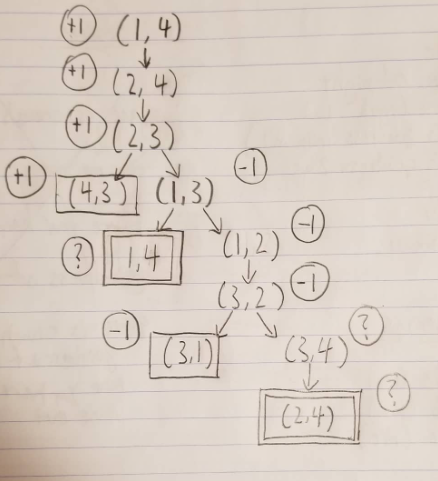
\includegraphics[width=\linewidth]{images/game_tree} \\
    "?" values are used to annotate loop states.
    When an agent has to choose between a +1 value and a "?" value (+1,?)
    the max player will always choose +1 while the min player will choose ?,
    and vice versa for (-1,?), with the min player choosing -1 and the max player choosing "?".
    Since the game value of a loop state is unknown, it is best for a max/min player to choose
    the corresponding max/min value if it is available, however if that value is not
    available the "?" state is a viable option to explore as it cannot be worse than an immediate loss.
    If all the successors of a state have a "?" value, the backed-up value is also "?".

    \begin{center}
        \Large
        \textbf{Problem 2}
    \end{center}
    \normalsize
    \begin{enumerate}
        \item[(a)] Computing the joint probability distribution:
            \begin{gather*}
                P(a, b, c, d, e) = P(a)*P(b)*P(c)*P(d|a,b)*P(e|b,c)\\
                P(a, b, c, d, e) = 0.2*0.5*0.8*0.1*0.3\\
                P(a, b, c, d, e) = 0.0024
            \end{gather*}
        \item[(b)] Computing the joint probability distribution:
            \begin{gather*}
                P(\neg{a}, \neg{b}, \neg{c}, \neg{d}, \neg{e}) = P(\neg{a})*P(\neg{b})*P(\neg{c})*P(\neg{d}|\neg{a},\neg{b})*P(\neg{e}|\neg{b},\neg{c})\\
                P(\neg{a}, \neg{b}, \neg{c}, \neg{d}, \neg{e}) = 0.8*0.5*0.2*0.1*0.8\\
                P(\neg{a}, \neg{b}, \neg{c}, \neg{d}, \neg{e}) = 0.0064
            \end{gather*}
        \item[(c)] Using the conditional probability rule $P(A|B) = \frac{P(A\bigcap B)}{P(B)}$
            \begin{gather*}
                P(\neg{a} | b, c, d, e) = \frac{P(\neg{a}, b, c, d, e)}{P(b, c, d, e)}\\
                P(\neg{a} | b, c, d, e) = \frac{P(\neg{a}, b, c, d, e)}{P(a, b, c, d, e) + P(\neg{a}, b, c, d, e)}\\
                P(\neg{a} | b, c, d, e) = \frac{P(\neg{a})*P(b)*P(c)*P(d|\neg{a},b)*P(e|b,c)}{0.0024 + P(\neg{a})*P(b)*P(c)*P(d|\neg{a},b)*P(e|b,c)}\\
                P(\neg{a} | b, c, d, e) = \frac{0.8*0.5*0.8*0.6*0.3}{0.0024 + 0.8*0.5*0.8*0.6*0.3}\\
                P(\neg{a} | b, c, d, e) = \frac{0.0576}{0.0024 + 0.0576}\\
                P(\neg{a} | b, c, d, e) = 0.96
            \end{gather*}
    \end{enumerate}

    \begin{center}
        \Large
        \textbf{Problem 3}
    \end{center}
    \normalsize
    \begin{enumerate}
        \item[(a)]
            \begin{gather*}
                P(b|j,m) = \alpha*P(b,j,m)\\
                \alpha = \frac{1}{P(\neg{b}, j, m) + P(b, j, m)}
            \end{gather*}
            \begin{gather*}
                P(b,j,m) = \sum_{e}\sum_{a}P(b,j,m,e,a)\\
                P(b,j,m) = P(b) \sum_{e} P(e) \sum_{a} P(a|b,e) P(j|a) P(m|a)\\
                P(b,j,m) =
                    0.001*0.002*0.95*0.9*0.7+
                    0.001*0.002*0.05*0.05*0.01+\\
                    0.001*0.998*0.94*0.9*0.7+
                    0.001*0.998*0.06*0.05*0.01\\
                P(b,j,m) = 0.00059224259\\
            \end{gather*}
            \begin{gather*}
                P(\neg{b},j,m) = \sum_{e}\sum_{a}P(\neg{b},j,m,e,a)\\
                P(\neg{b},j,m) = P(\neg{b}) \sum_{e} P(e) \sum_{a} P(a|\neg{b},e) P(j|a) P(m|a)\\
                P(\neg{b},j,m) =
                    0.999*0.002*0.29*0.9*0.7+
                    0.999*0.002*0.71*0.05*0.01+\\
                    0.999*0.998*0.001*0.9*0.7+
                    0.999*0.998*0.999*0.05*0.01\\
                P(\neg{b},j,m) = 0.00149185764
            \end{gather*}
            \begin{gather*}
                \alpha = \frac{1}{P(\neg{b}, j, m) + P(b, j, m)}\\
                \alpha = \frac{1}{0.00149185764 + 0.00059224259}\\
                \alpha = \frac{1}{0.00208410023}\\
            \end{gather*}
            \begin{gather*}
                P(b|j,m) = \alpha*P(b,j,m)\\
                P(b|j,m) = \frac{0.00059224259}{0.00208410023}\\
                P(b|j,m) = 0.28417183659
            \end{gather*}
        Therefore, the probability of a burglary given that John and Mary both called, is
        $0.28417183659$.
        \item[(b)] In a Bayesian network in the form of a chain, using the enumeration
        method has a worst case runtime of $\mathcal{O}(2^n)$, as moving down each level
        in the chain generates another level in a binary tree.\\

        Using the variable elimination method, moving down each level in the Bayesian network
        chain only adds one additional problem to compute (point-wise product of factors), as each node in the
        network only has one parent.
        Thus, the variable elimination method has a worst case
        runtime of $\mathcal{O}(n)$.
    \end{enumerate}

    \begin{center}
        \Large
        \textbf{Problem 4}
    \end{center}
    \normalsize
    \begin{enumerate}
        \item[(a)]
        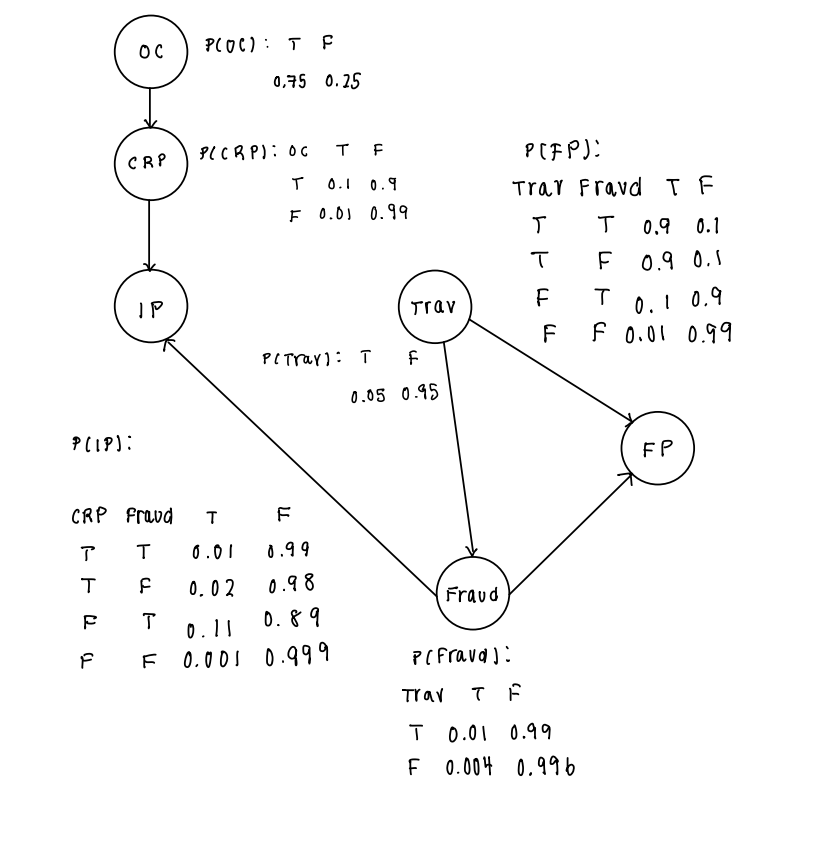
\includegraphics[width=\linewidth]{images/bayesnetwork} \\
        \item[(b)]
        Probability the current transanction is a fraud prior to searching for previous computer related purchases and before verifying if it is a foreign and/or an internet purchase:\\
        \begin{gather*}
        P(Fraud) = \\P(Fraud = True| Trav = True) * P(Trav = True) + \\P(Fraud = True| Trav = False) * P(Trav = False) =\\ 0.01 * 0.05 + 0.004 * 0.95 = \\0.0043\\
        \end{gather*}
        \\
        
        Probability the current transaction is a fraud given that it is a foreign transaction, not an internet purchase, and card holder purchased computer related purchases in the past week:\\
        \begin{gather*}
        P(Fraud = True| IP = False, CRP = True, OC = True) =\\ P(IP = False| CRP = True, Fraud = True) * P(CRP = True) +\\ P(IP = False| CRP = False, Fraud = True) * P(CRP = False) =\\ P(IP = False| CRP = True, Fraud = True) * (P(CRP = True| OC = True) *\\ P(OC = True) +\\ P(CRP = True| OC = False) * P(OC = False)) +\\ P(IP = False| CRP = False, Fraud = True) * (P(CRP = False| OC = True) *\\ P(OC = True) +\\ P(CRP = False| OC = False) * P(OC = False)) =\\ 0.99 * (0.1 * 0.75 + 0.01 * 0.25) + 0.89 * (0.9 * 0.75 + 0.99 * 0.25) =\\ 0.89775\\
        \\
        P(Fraud = True| FP = True) =\\ P(Fraud = True| Trav = True) * P(FP = True| Trav = True, Fraud = True) *\\ P(Trav = True) +\\ P(Fraud = True| Trav = False) * P(FP = True| Trav = False, Fraud = True) *\\ P(Trav = False) =\\ 0.01 * 0.90 * 0.05 + 0.004 * 0.10 * 0.95 =\\ 0.00083\\
        \\
        P(Fraud = True | IP = False, CRP = True, OC = True, FP = True) =\\ 0.89775 * 0.00083 =\\ 0.000745\\
        \end{gather*}
    \end{enumerate}

\end{document}
